\documentclass{beamer}
\usetheme{focus}

\usepackage{amsmath}
\usepackage{braket}

\definecolor{main}{RGB}{92, 138, 168}
\definecolor{background}{RGB}{240, 247, 255}

\title{Implementazione di un algoritmo KNN multiclasse su hardware quantistico}
\subtitle{Tesi di laurea in fisica}
\author{Mariano Mollo N85000880\texorpdfstring{\\}{,} Relatore: Giovanni Acampora}
\titlegraphic{
\includegraphics[scale=0.15]{gfx/logo-federico-II-blu}}
% ********************************************************
% Prova a mettere la trasparenza
% ********************************************************
\institute{Università degli Studi di Napoli Federico II}
\date{15 ottobre 2019}

\begin{document}
	\begin{frame}
		\maketitle
	\end{frame}

	\begin{frame}{Indice}
		\begin{enumerate}
			\item Introduzione
			\item Machine learning
			\item Quantum computing
			\item Metodi
			\item Quantum machine learning
			\item Risultati
			\item Conclusione
		\end{enumerate}
	\end{frame}

	\section{Introduzione}

	\begin{frame}
		\frametitle{Machine learning}
	
		Il machine learning dà l'abilità ai computer di apprendere dai dati

		Gli algoritmi di machine learning prevedono spesso

		\begin{itemize}
			\item risolvere grandi sistemi di equazioni lineari
			\item invertire grandi matrici
			\item calcolo di distanze
		\end{itemize}
	
		Effettuare queste operazioni su grandi insiemi di dati diventa 
		man mano più difficoltoso
	\end{frame}

	\begin{frame}
		\frametitle{Quantum computing}
	
		Costruire hardware di elaborazione basandosi sulla meccanica quantistica

		\begin{itemize}
			\item La meccanica quantistica si occupa di vettori in spazi di Hilbert
			\item I computer quantistici eseguono operazioni lineari su qubit
			\item Sistemi a molti qubit sono descritti da grandi vettori che possono 
			essere manipolati in parallelo sui computer quantistici 
			\item Il machine learning prevede la manipolazione di grandi vettori e matrici
		\end{itemize}
	
	\end{frame}

	\begin{frame}
		\frametitle{Quantum machine learning}
	
		Permette ai quantum computer di imparare dai dati più velocemente dei computer classici
	
	\end{frame}

	\section{Machine learning}

	\begin{frame}
		\frametitle{Machine learning supervisionato}
	
		Posto un insieme dati di input con i corrispondenti output, 
		si predica l'output di nuovo input sconosciuto. 
	
	\end{frame}

	\begin{frame}
		\frametitle{k-nearest neighbours classico pesato sulla distanza}
	
		k è un numero naturale

		Dato un dataset D = v0, ..., vn

		Dato un nuovo vettore x: 

		si considerino i k vettori più vicini ad x 

		si classifichi x con un voto a maggioranza 

		Si assegni pesi dipendenti dall'inverso della distanza per 
		aumentare l'influenza di quelli più vicini
	
	\end{frame}

	\section{Quantum computing}

	\begin{frame}
		\frametitle{Bit classici e bit quantistici (qubit)}
	
		% immagine *************************

		Bit classico

		\begin{itemize}
			\item Implementato di solito usando MOSFET\footnote{Metal oxide semiconductor field effect transistor}
			\item 2 stati definiti (0, 1)
			\item Può essere o 0 o 1
		\end{itemize}
	
	\end{frame}

	\begin{frame}
		\frametitle{Bit classici e bit quantistici (qubit)}
	
		% immagine *************************

		Bit quantistico (qubit)

		Può essere |0> o |1>

		Può essere anche |0> e |1> contemporaneamente (sovrapposizione quantistica)
	
	\end{frame}

	\begin{frame}
		\frametitle{Il qubit}
	
		Matematicamente, la sovrapposizione di un qubit è espressa come 

		\begin{equation*}
			\ket{\psi} = \alpha \ket{0} + \beta \ket{1} \cong \begin{pmatrix}
				\alpha \\ \beta
			\end{pmatrix}
		\end{equation*}

		dove alfa e beta sono complessi e sono chiamati ampiezze di probabilità. 

		L'ultima espressione è chiamata vettore ampiezza. 
	
	\end{frame}

	\begin{frame}
		\frametitle{Stato dell'arte del quantum computing}
	
		IBM 14 qubit superconduttivi

		Google 9 qubit superconduttivi (al 2017)

		Weizmann Research Group in Israele 8 ioni intrappolati (al 2017)

		DWave 1152 qubit ma è limitato (al 2017)
	
	\end{frame}

	\begin{frame}
		\frametitle{Sistemi a molti qubit}
	
		Un computer quantistico con $n$ qubit possiede $2^n$ ampiezze di probabilità

		Queste ampiezze possono essere usate per immagazzinare quantità enormi di informazioni

		Numero di qubit | RAM classica richiesta | tempo di simulazione

		5 | 256 byte | secondi su un cellulare
		25 | 2 gigabyte | secondi su un portatile
		50 | 8000 terabyte | secondi su un supercomputer
		275 | numero di atomi nell'universo osservabile | età dell'universo
		
	\end{frame}

	\begin{frame}
		\frametitle{Motivazione}
	
		Si vuole mostrare come rendono gli algoritmi di quantum machine 
		learning all'aumentare del numero di qubit utilizzati su hardware reale
	
	\end{frame}

	\section{Metodi}

	\begin{frame}
		\frametitle{IBM Quantum Experience}
	
		\begin{itemize}
			\item Accessibile al pubblico
			\item Permette simulazioni con o senza rumore
			\item Fino a 14 qubit superconduttivi
			\item Fino a 32 qubit simulati
		\end{itemize}
		
	
	\end{frame}

	\begin{frame}
		\frametitle{Qiskit}
	
		Piccoli quantum computer possono essere simulati su computer convenzionali

		Qiskit permette di 

		\begin{itemize}
			\item ideare circuiti quantistici
			\item simularne l'esecuzione sul proprio pc
			\item interfacciarsi con l'IBM QX
			\item mandare ordini di esecuzione a veri computer quantistici
		\end{itemize}
	
	\end{frame}

	\section{Quantum machine learning}

	\begin{frame}
		\frametitle{Codificare i dati nelle ampiezze}
	
		Si è usata la costruzione di una QRAM (Quantum RAM) attraverso 
		l'algoritmo di costruzione di Petruccione et al. per 
		codificare vettori classici nei vari stati quantistici 
		a disposizione

		\begin{equation*}
			\text{QRAM} \ket{0} = \ket{\psi}
		\end{equation*}
	
	\end{frame}

	\begin{frame}
		\frametitle{QKNN}
	
		Stato quantistico iniziale

		\begin{equation*}
			\ket{\psi_0} = \frac{1}{\sqrt{2M}} \sum_{m=1}^M 
			(\ket{0}\ket{\psi_x}+\ket{1}\ket{\psi_{t^m}})\ket{c^m}\ket{m}
		\end{equation*}

		Calcolo della distanza con interferenza quantistica

		\begin{equation*}
			\ket{\psi_1} = \frac{1}{2\sqrt{M}}\sum_{m=1}^M 
			(\ket{0}(\ket{\psi_x}+\ket{\psi_{t^m}})+\ket{1}(\ket{\psi_x}-\ket{\psi_{t^m}}))\ket{c^m}\ket{m}
		\end{equation*}
	
		Misura condizionale

		\begin{equation*}
			\ket{\psi_2} = \frac{1}{2\sqrt{M}} \sum_{m=1}^M \sum_{i=1}^N
			(x_i+t_i^m)\ket{0}\ket{i}\ket{c^m}\ket{m}
		\end{equation*}

		

	\end{frame}

	\begin{frame}
		\frametitle{QKNN}
	
		Probabilità di misurare una data classe

		\begin{equation*}
			P(\ket{c^m} = \ket{s}) = \sum_{m|c^m=s} 
			1 - \frac{1}{4M} |x-t^m|^2
		\end{equation*}

		Classificazione

		\begin{equation*}
			c = \begin{cases}
			0 \quad se P(\ket{c^0}) maggiore \\
			1 \quad se P(\ket{c^1}) maggiore \\
			etc\ldots
		\end{cases}
		\end{equation*}
	
	\end{frame}

	\section{Risultati}

	\begin{frame}
		\frametitle{Data set Iris}
	
		L'insieme dati usato per far girare l'algoritmo 
		è stato il ben noto Iris Data Set

		Si è prima standardizzato e normalizzato i vettori 
		di training e poi si è proceduto alla classificazione
		
		\begin{figure}[]
			\centering
			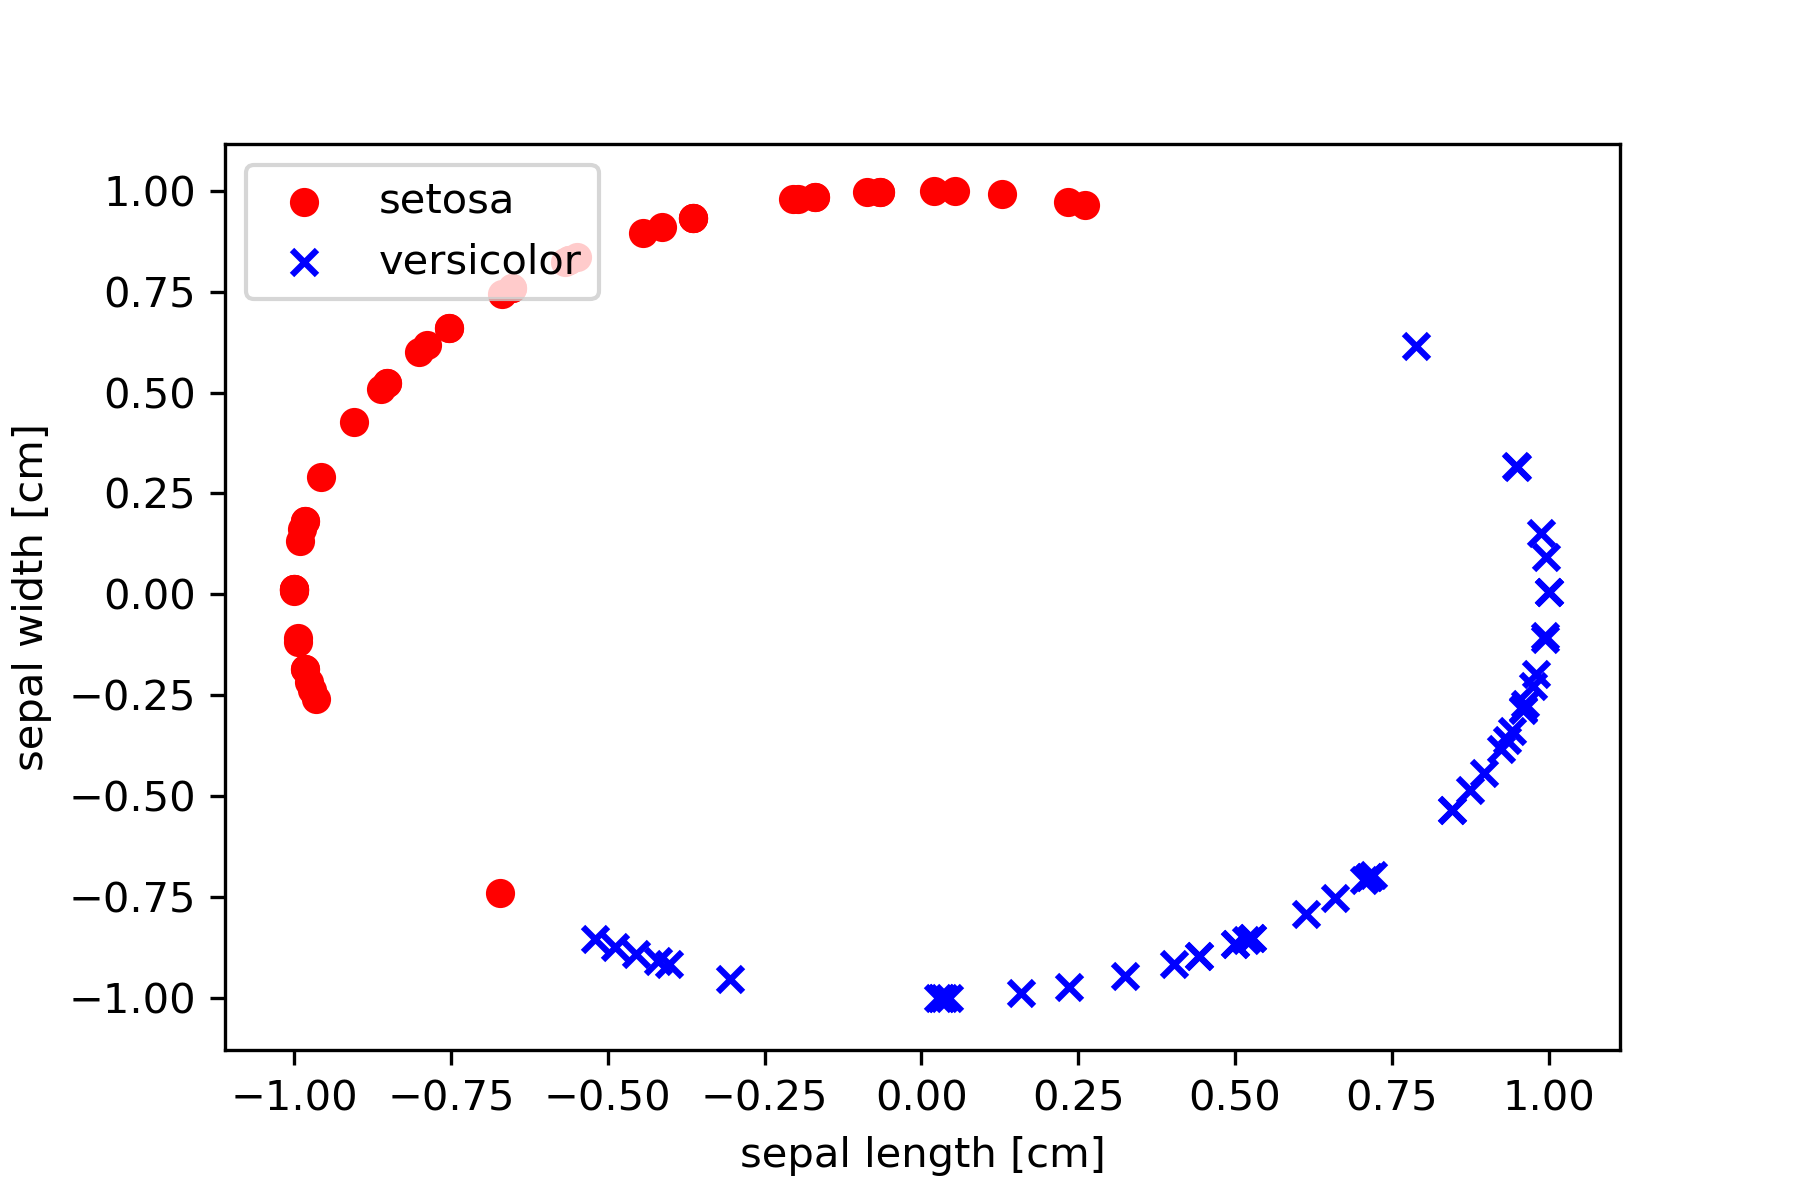
\includegraphics[width=.75\textwidth]{gfx/iris/iris2normalized}
			\caption{}
			\label{fig:iris_normalizzato}
		\end{figure}

	\end{frame}

	\begin{frame}
		\frametitle{Simulazioni}
		\begin{figure}[]
			\centering
			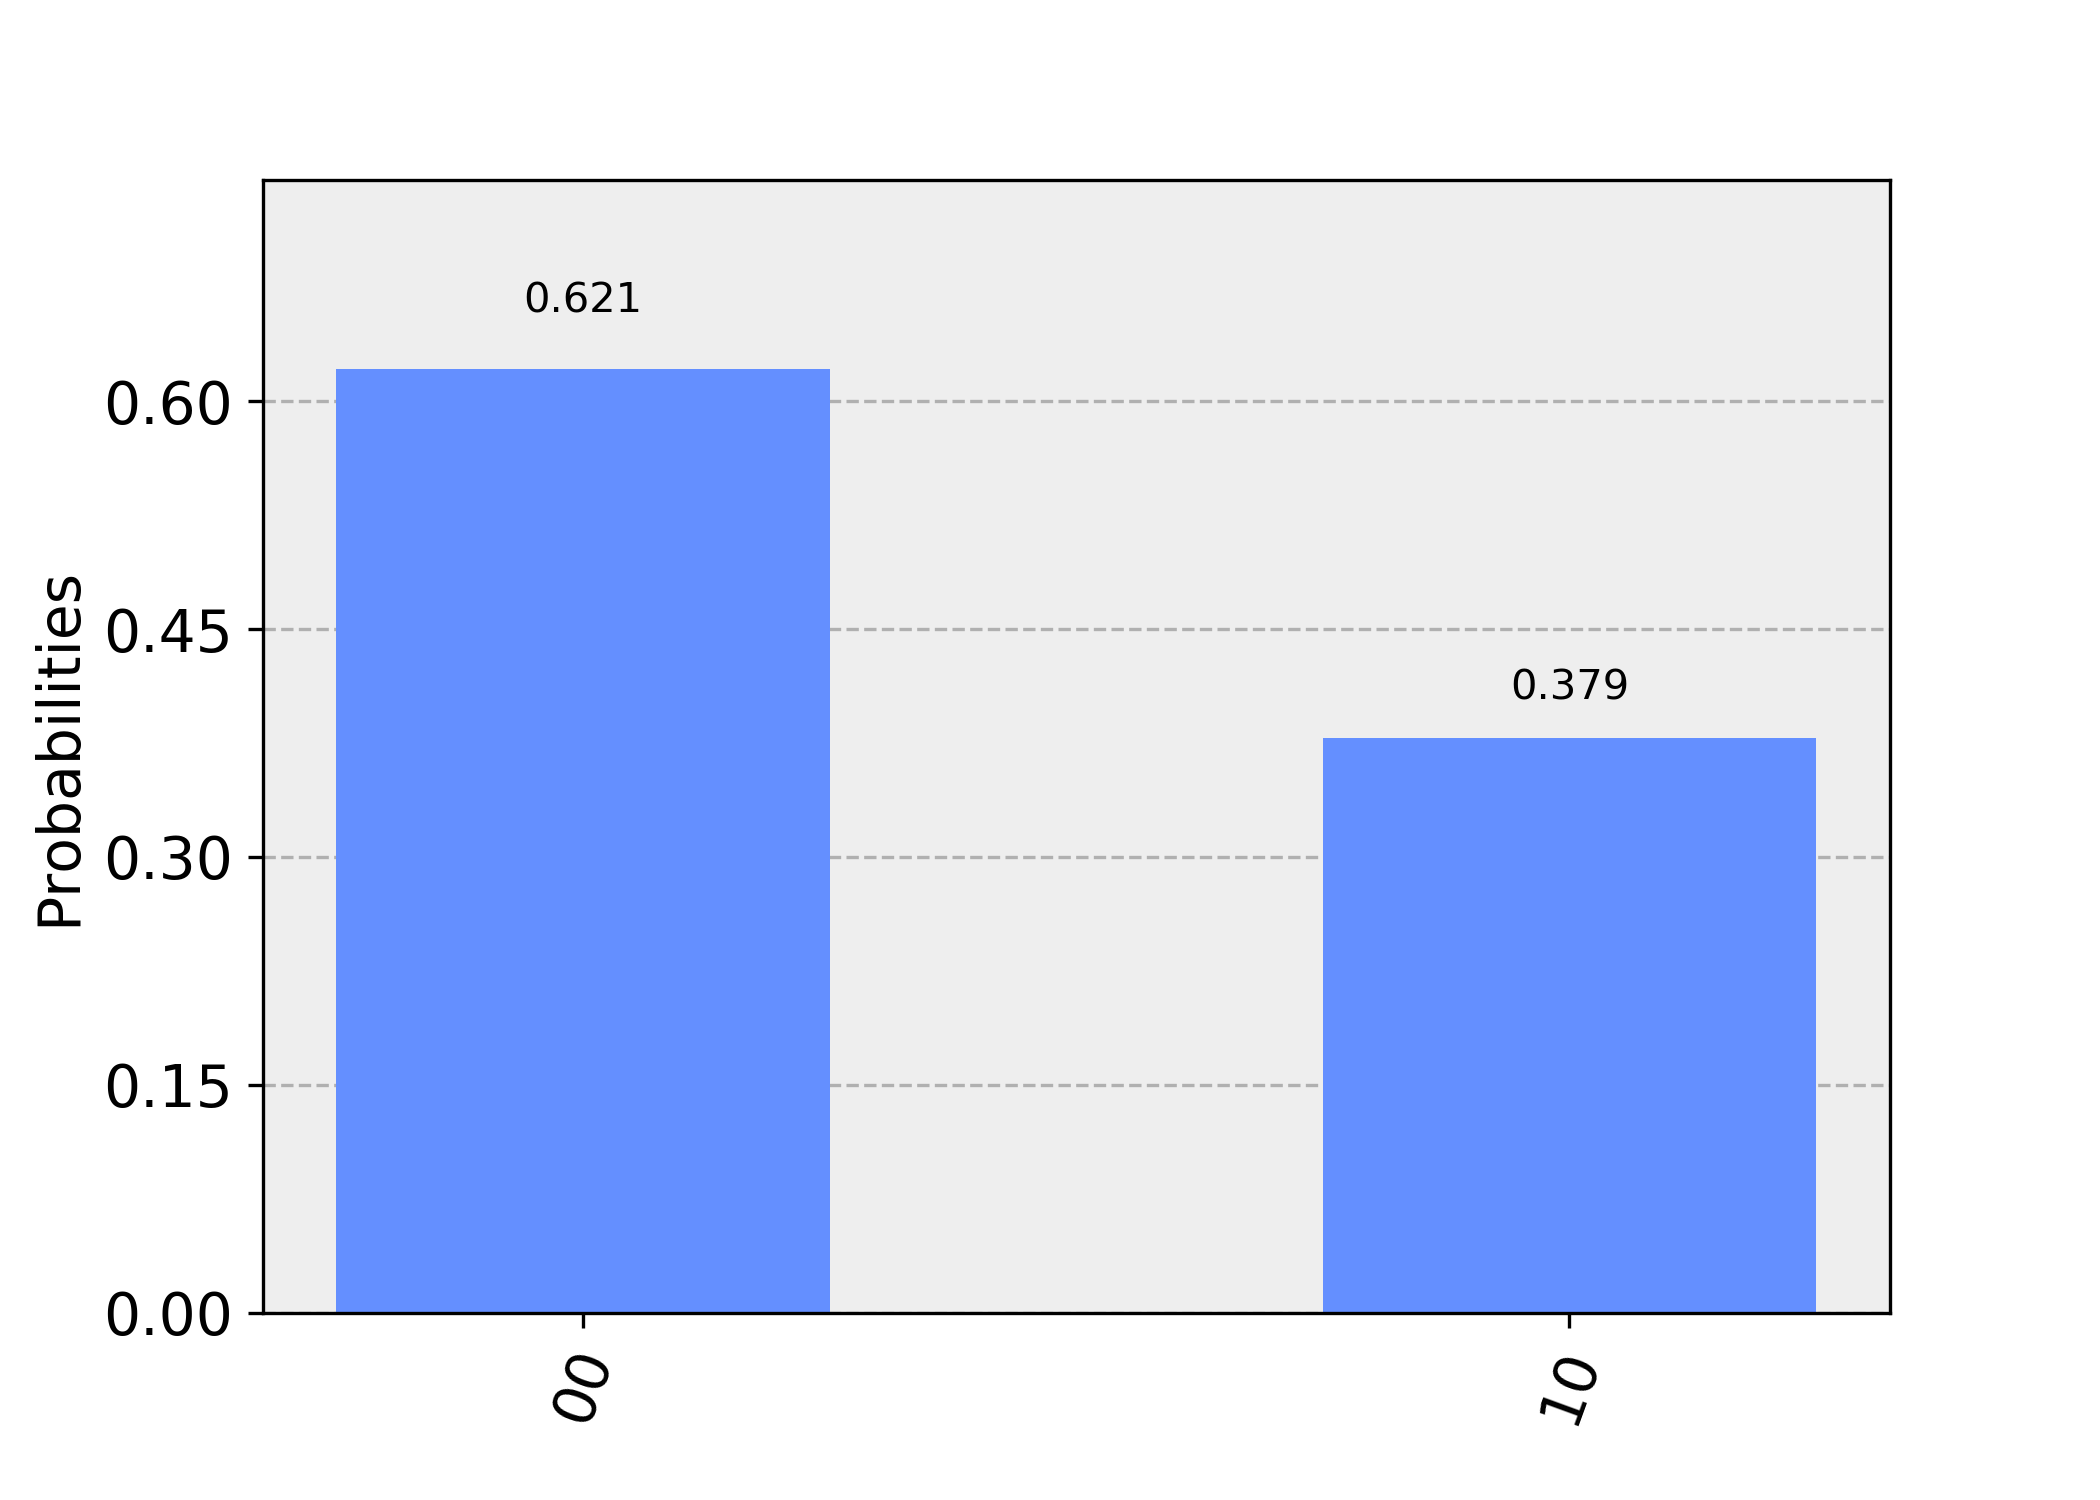
\includegraphics[width=\textwidth]{gfx/iris/histogram}
			\caption{}
			\label{fig:setosa_simulazione}
		\end{figure}
	
	\end{frame}

	\begin{frame}
		\frametitle{Esecuzioni reali}
		\begin{figure}[]
			\centering
			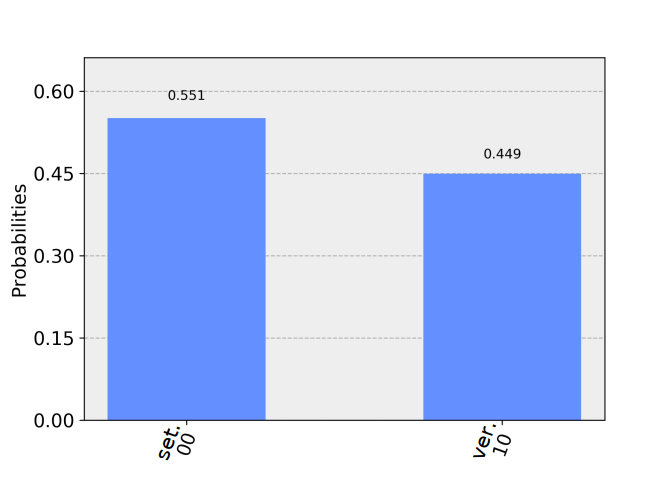
\includegraphics[width=\textwidth]{gfx/misura_setosa_sperimentale}
			\caption{}
			\label{fig:setosa_sperimentale}
		\end{figure}
	\end{frame}
\end{document}
